%%%%%%%%%%%%%%%%%%%%%%%%%%%%%%%%%%%%%%%%%%%%%%%%%
%%%%%%%%%%%%%%%%%%%%%%%%%%%%%%%%%%%%%%%%%%%%%%%%%

\chapter{Foraging}
\label{chap:second}

%%%%%%%%%%%%%%%%%%%%%%%%%%%%%%%%%%%%%%%%%%%%%%%%%
%%%%%%%%%%%%%%%%%%%%%%%%%%%%%%%%%%%%%%%%%%%%%%%%%

In swarm robotics, robot foraging has become a benchmark problem due to its complex nature involving the coordination of numerous sub-tasks. Robot foraging is also one of the swarm robotics problems that has some very obvious useful applications. This chapter aims to provide an in-depth review of what foraging is, how different social insects forage as well as to provide a review of existing foraging algorithms in swarm robotics. The definition of foraging in swarm robotics is discussed in Section~\ref{sec:second:definition}, while Section~{foraginginnature} describes foraging behaviours observed in nature, specifically in bees and ants. Section~\ref{biological:ants} provides a taxonomy of the types of swarm robotic foraging algorithms, and the challenges that foraging algorithms must address are discussed in Section~\ref{challengesinforaging}. Existing swarm robotics foraging algorithms are outlined in Section~\ref{sec:second:existingsolution} , and prioritized foraging is defined and discussed in Section~
\ref{sec:second:prioritizedforaging}. Lastly, the chapter is summarized in Section~\ref{foraging:summary}. 


%%%%%%%%%%%%%%%%%%%%%%%%%%%%%%%%%%%%%%%%%%%%%%%%%
%%%%%%%%%%%%%%%%%%%%%%%%%%%%%%%%%%%%%%%%%%%%%%%%%

\section{Definition}
\label{sec:second:definition}

Foraging was initially studied by biologists, particularly the foraging behaviour of ants \cite{holldobler1990ants,bernstein1974seasonal}, bees \cite{seeley2009wisdom} and bacteria \cite{resnick1994turtles}. Foraging has a variety of real-life applications such as search and rescue \cite{jennings1997cooperative,murphy2000biomimetic}, and waste clean-up \cite{balch1995io}. Numerous swarm robotics algorithms have been developed to improve robustness, time and energy efficiency of the foraging process for multiple variations of the foraging problem as outlined in \cite{winfield2009foraging}. 

Foraging is the act of searching for and collection (or capturing) food for storage and consumption \cite{winfield2009foraging}. Foraging is an important problem that was first addressed by biologists in the examination of nature, particularly with the foraging behaviour of ants and bacteria. In a robot context, foraging is defined as the search and collection of scattered objects in an environment and returning those objects to a collection point.

The foraging sub-tasks involve the efficient search and collection of food, homing whilst carrying food to the nest site, and then depositing of the food item in the nest before returning to the foraging task. Efficient foraging requires indirect or direct co-operation between individuals, in order to transport food items too large for individual transport. The foraging process has been adapted for numerous foraging problems and for different types of robots.


\section{Foraging in Nature}
\label{foraginginnature}
As with many swarm robotics problems, the inspiration for foraging comes from nature, in particular, social insects such as ants and honey bees. This section describes the biological inspiration for foraging.


\subsection{Ants}
\label{biological:ants}
% Intro 
As with many swarm robotics problems, the inspiration for foraging comes from nature, in particular, social insects such as ants and honey bees. This section describes the biological models that are used in the algorithms derived by this thesis. 

%Ants
The study of ants has revealed that impressive emergent activities can be achieved with simple interacting agents with only a few simple rules. Ants use a form of communication known as stigmergy \cite{dorigo2000ant}. Ants perform indirect communication between ants by depositing a substance known as pheromone. In foraging, pheromone is deposited on the paths between the nest and the food source. Other ants detect the deposited pheromone and will prefer to follow paths which have a greater amount of pheromone deposit. Ant pheromones have been modelled in numerous swarm intelligence algorithms such as ant colony optimization and ant systems \cite{dorigo2006ant, dorigo2010ant}. 
 
Although algorithms based on ant foraging behaviour are used to solve optimization problems, the algorithms are often difficult to replicate in a real-life robotic environment since most of the algorithms need to model pheromone dropping and detection. A robotics algorithm that uses pheromone requires robots to be equipped with a substance-distributors, beacon-deployers or complex communication that simulates pheromone deposition and trail-following \cite{hoff2010two}.

The desert ant (\textit{Cataglyphis fortis}) does not make use of stigmergy to forage, as pheromone deposited on desert sand would be blown away by the wind \cite{collett1992visual}. Instead, desert ants use a technique called path integration for navigation to relocate food sources that have already been found by random exploration \cite{collett1998local,wehner2003desert}. Fig~\ref{pathintegration} demonstrates path integration. The black solid lines represent the path of the ant and the blue dotted lines show how the direction to the nest is maintained as the ant explores. The ant is constantly monitoring the change in heading from the original heading such that at the destination the ant has a direction directly back to the sink. As a result, a shortcut back to the nest is calculated in order to minimize heat stress. The shortcut back to the nest is known as the home vector \cite{muller1988path}. Path integration, more commonly known as dead reckoning, is a key evolutionary aspect gained from living in the hot barren desert. When path integration fails, the ant resorts to using landmarks, such as the sun, for navigation \cite{collett1998local}.

\begin{figure} [h]
	\centering
	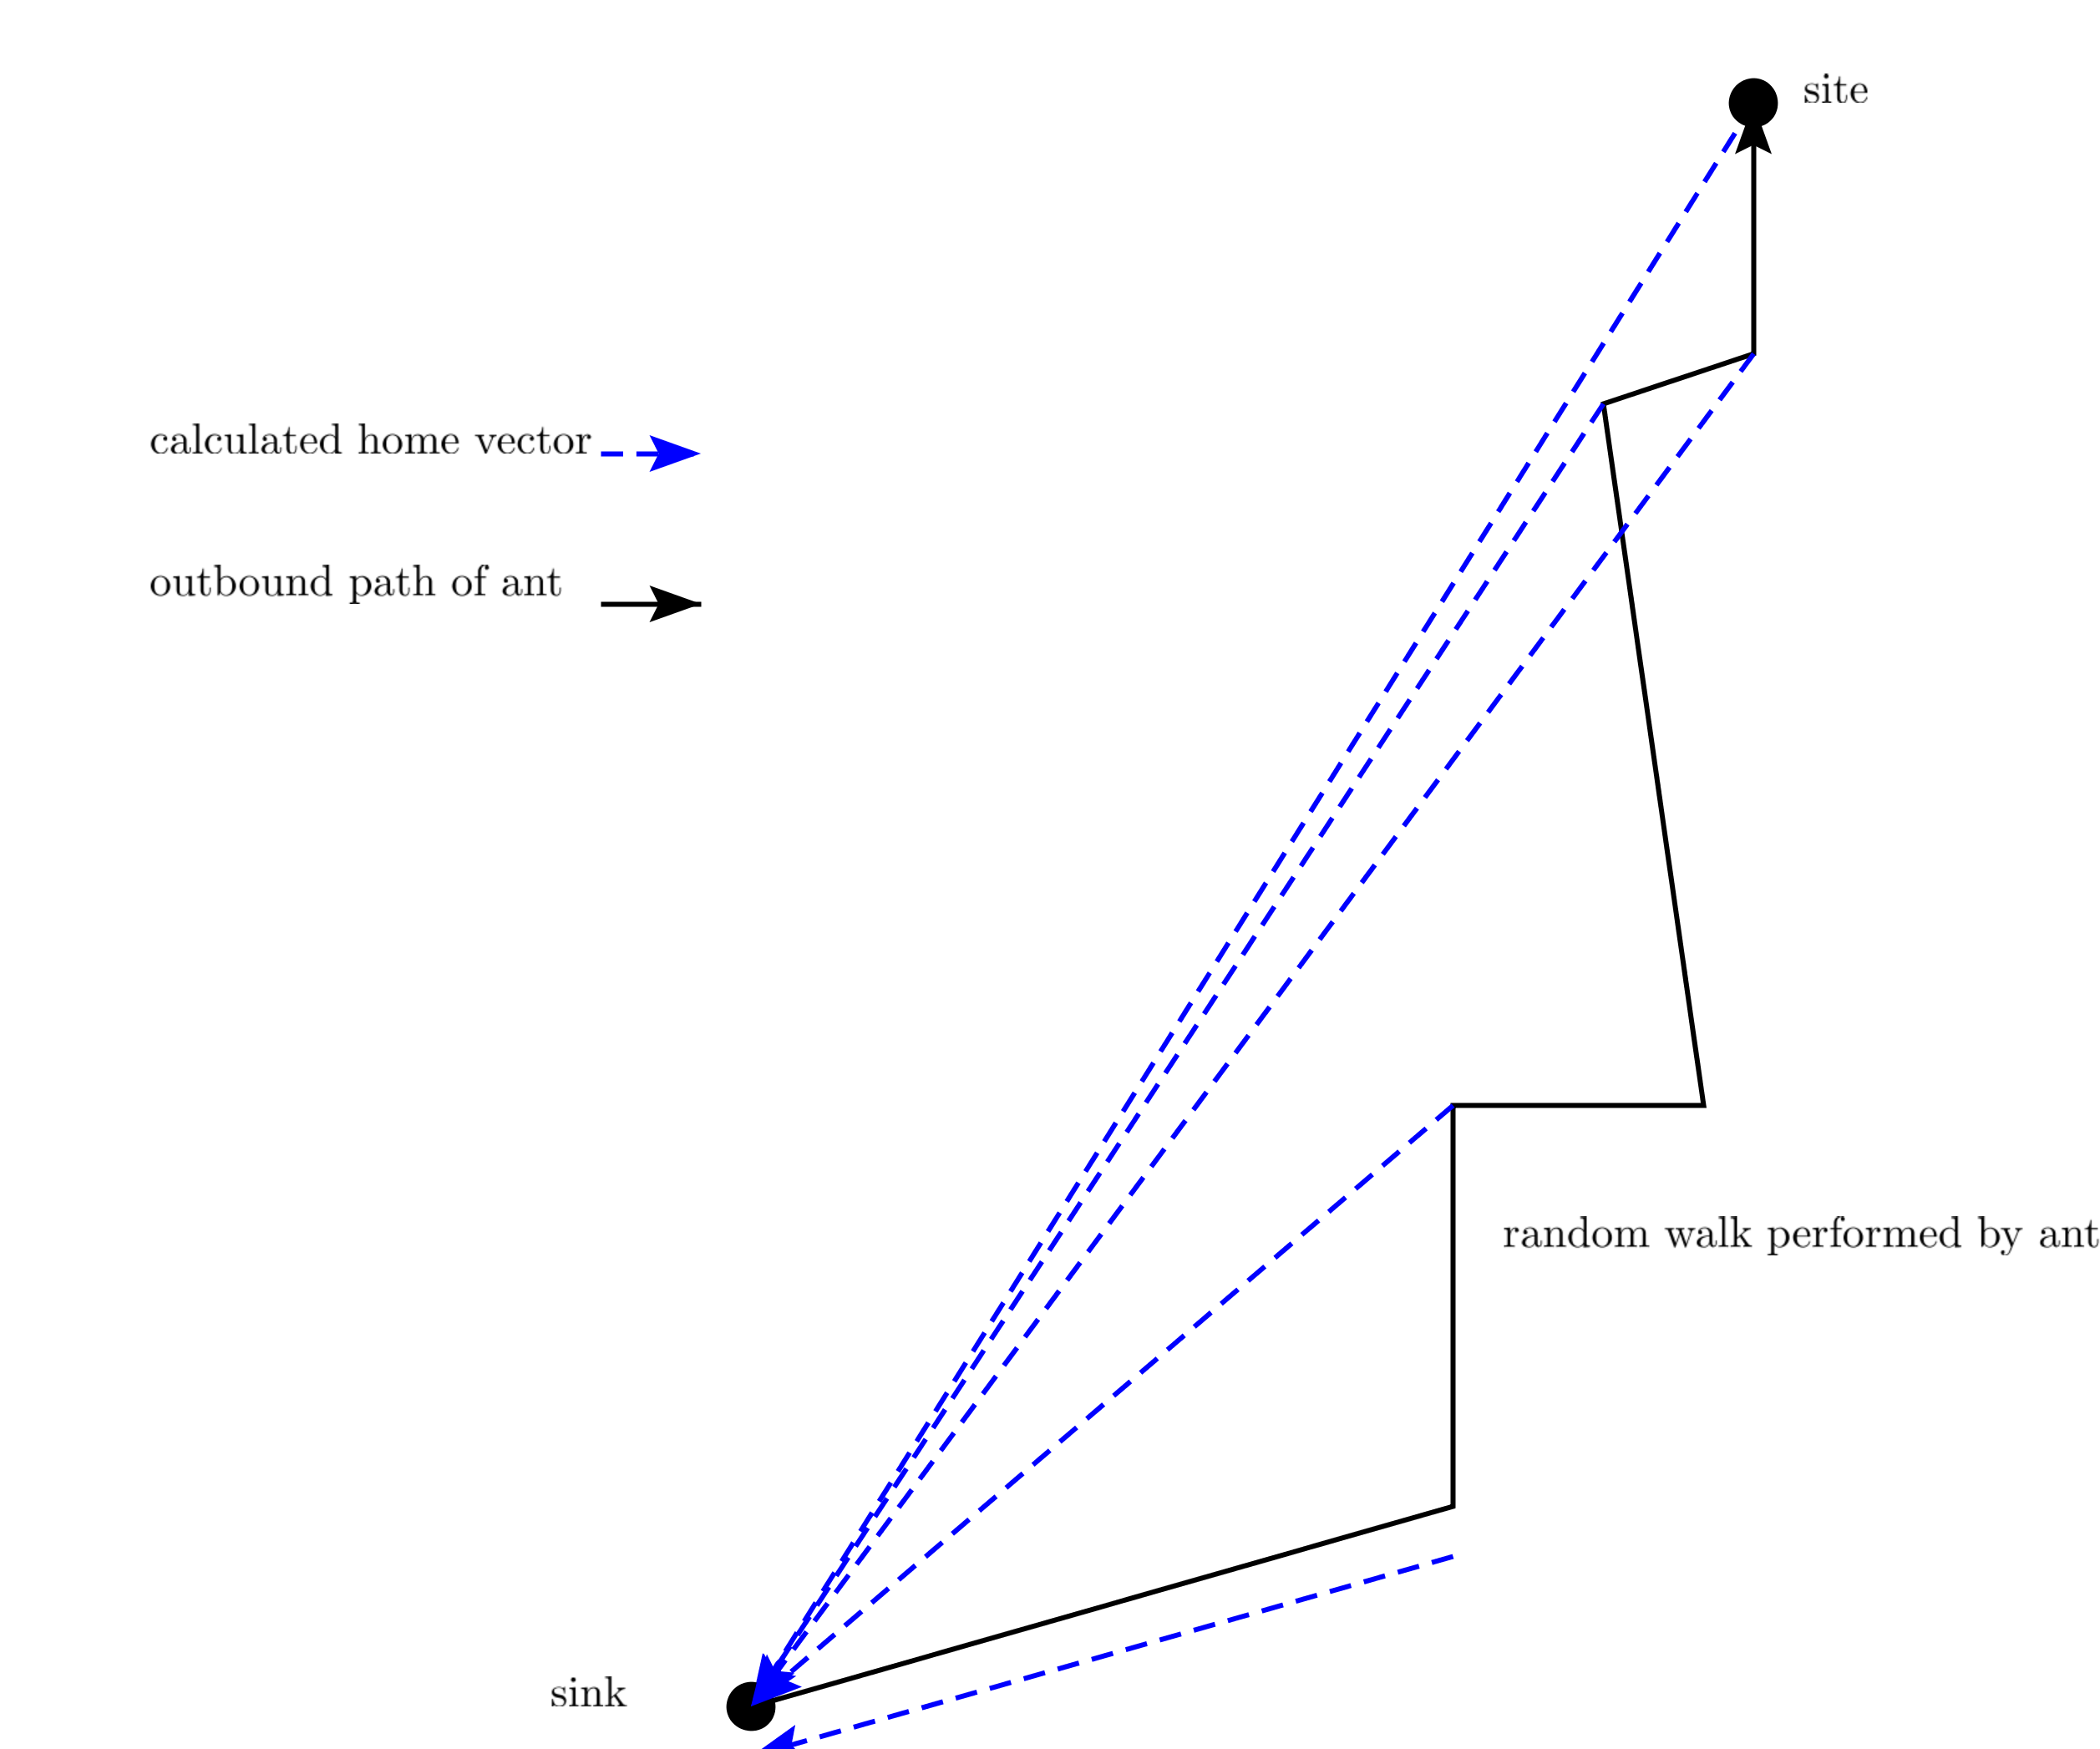
\includegraphics[width=\textwidth]{chapters/chapter2/figures/drawing.png}
	\caption{Path Integration }
	\label{pathintegration}
\end{figure}

Due to the lack of pheromone, the desert ant is thus simpler to model for real-robot interaction. Desert ant foraging has been modelled in \cite{moller1998modeling,hecker2012formica}. Hecker et al \cite{hecker2012formica} performed experiments to compare the performance of two foraging algorithms algorithms: The one algorithm was based on the desert ant foraging which has no pheromone-like communication and the other used including pheromone-like communication. It was shown that communication improved performance; however, the desert-ant algorithm still performed comparatively well. 

\subsection{Bees}
\label{bees:biologicalinspiration}
Bees have an impressive set of abilities considering the simplicity of a single individual. They have the ability to remember the colour and shape of flowers \cite{zhang2006honeybee}, and in terms of navigation, they are able to learn local features and routes due to well-developed learning and memorizing capacities \cite{menzel2001cognitive}. Honey-bees are even time aware \cite{moore1989influence}. 

Honey bees have efficient division of labour between different functions in the hive, such as foraging and brood-care. Within the foraging activity itself, honey bees perform foraging-specific division of labours. Honey bee foraging is made up of three different roles namely employed foraging, unemployed foraging and scouting \cite{seeley2009wisdom}. Scouts explore the environment to locate new food sources. Once a source has been found, scouts return to the hive to communicate information about the located food source. To communicate the foraging information, scout bees perform a waggle-dance at the hive. The waggle-dance communicates information about the distance and bearing of the resource. The communication of a good foraging site is known as recruitment \cite{seeley2009wisdom}.

Unemployed foragers wait on the dance floor, and evaluate the dances of the scout bees. An unemployed bee select a location described by the scout bees, and become an employed forager. Employed forager bees use the information about the resource, attempt to locate the source, load themselves with food, and return to the hive where unemployed foragers are ready to offload the food. Jansen \cite{janson2007searching} suggests that unemployed bees become exploring scouts when they do not detect any dancing scout bees. 

\subsection{Bacteria}

The $E. coli$ bacteria forage for carbohydrates in the human gut. The bacteria have a unique search mechanism whereby they move in the same direction for a period of time (which is called a "run") and then change direction using their complex flagella (known as a "tumble"). The bacteria exhibit the behaviour continuing to move in a direction, if the bacteria are moving up a nutrient gradient. Bacteria stop moving in a direction, if they're moving down a nutrient gradient in order to avoid toxic substances. Under certain conditions, the bacteria secrete an attractant substance which attracts the bacteria to one another for protection.

The foraging behaviour of $E. coli$ bacteria is used for inspiration for a computational intelligence algorithm \cite{passino2010bacterial} and particle swarm optimization is, for instance based on the flocking behaviour of birds - a flocking behaviour exhibited when finding food, amongst other things \cite{kennedy1995particle}. 

\subsection{Predator Prey}

Predator prey scenarios are foraging problems where the items to be foraged actively avoid capture (known as prey)  and the animals pursuing the prey are known as predators \cite{winfield2009foraging}. Predator prey foraging has been extensively studied in the field of Optimal Foraging Theory, which aims to predict the behaviour of an animal searching for food \cite{charnov1976optimal}. 

% TODO: Quote some of the examples of how certain predators capture certain prey.

Predator-prey  models have been used in other swarm intelligence techniques in multi-objective optimization problems \cite{nolfi1998coevolving}.

\section{Foraging in Swarm Robotics}
The following section addresses foraging in a swarm robotics context. Firstly, a taxonomy of robot foraging is presented and then existing nature-inspired swarm robotics foraging algorithms are discussed.

\subsection{Taxonomy of Robot Foraging}
\label{sec:second:taxonomy}

Foraging is a popular problem due to the vast potential opportunity of foraging for application to a variety of real-world problems from search and rescue \cite{jennings1997cooperative} to toxic waste retrieval to mining. It is beneficial to present a taxonomy of robot foraging that can be used to classify existing research about foraging as well as contextualize the specific foraging problems addressed by this thesis. One should note that the foraging taxonomy presented also includes non-swarm robotic foraging.

Multiple taxonomies have been developed as robot foraging research has progressed \cite{oster1978caste,ostergaard2001emergent}. However a more recent and complete foraging taxonomy is presented in \cite{winfield2009foraging}. The taxonomy classifies foraging solutions based on four major axes: the foragi ng environment, the capabilities and types of robots used for foraging, performance aspects, and the foraging strategy used in a foraging algorithm. Each of these major axes have a number of minor axes which are outlined in Table~\ref{foragingtaxonomytable_part1} and Table~\ref{foragingtaxonomytable_part2}.  The following sections discuss each of the major and minor axes in more detail

\begin{table}
\centering
    \caption{Winfield's Robot Foraging Taxonomy \cite{winfield2009foraging}}
    \label{foragingtaxonomytable_part1}
    
\begin{tabular}{ | c | c | c |}
	\hline
	Major Axis & Minor Axis & Value  \\ \hline
	\multirow{13}{*}{Environment}
		& \multirow{2}{*}{Search space} 
			& Unbounded \\  
		& 	& Constrained \\ \cline{2-3}
		& \multirow{3}{*}{Source Areas} 
			& Single limited \\ 
		&	& Single unlimited \\
		&	& Multiple \\ \cline{2-3}
		& \multirow{2}{*}{Sinks} 
			& Single \\
		&	& Multiple \\ \cline{2-3}
		& \multirow{3}{*}{Object types} 
			& Single static \\
		&	& Multiple static \\
		&	& Single active \\ \cline{2-3}
		& \multirow{3}{*}{Object placement} 
			& Fixed known locations \\
		&	& Uniform Distributions \\
		&	& Clustered \\\hline
	\multirow{16}{*}{Robot(s)}
		& \multirow{2}{*}{Number} 
			& Single \\  
		& 	& Multiple \\ \cline{2-3}
		& \multirow{3}{*}{Type} 
			& Homogenous \\ 
		&	& Heterogenous \\ \cline{2-3}
		& \multirow{2}{*}{Object Sensing} 
			& Limited range \\
		&	& Unlimited range\\ \cline{2-3}
		& \multirow{3}{*}{Localization} 
			& None \\
		&	& Relative \\
		&	& Absolute \\ \cline{2-3}
		& \multirow{3}{*}{Communications} 
			& None \\
		&	& Near \\
		&	& Infinite \\\cline{2-3}
		& \multirow{3}{*}{Power} 
			& Limited \\
		&	& Forage \\
		&	& Unlimited \\\hline
\end{tabular}
\end{table}

\begin{table}
\centering
    \caption{Winfield's Robot Foraging Taxonomy Part 2 \cite{winfield2009foraging}}
    \label{foragingtaxonomytable_part2}
    
\begin{tabular}{ | c | c | c |}
\hline
	Major Axis & Minor Axis & Value  \\ \hline
	\multirow{6}{*}{Performance}
		& \multirow{3}{*}{Time} 
			& Fixed \\  
		& 	& Minimum \\ 
		& 	& Unlimited \\ \cline{2-3}
		& \multirow{3}{*}{Energy} 
			& Fixed \\ 
		& 	& Minimum \\ 
		&	& Unlimited \\ \hline
	\multirow{6}{*}{Strategy}	
		& \multirow{5}{*}{Search} 
			& Limited range \\
		&	& Geometrical pattern\\
		&	& Trail following\\
		&	& Follow other robots\\
		&	& In teams\\ \cline{2-3}
		& \multirow{2}{*}{Grabbing} 
			& Single \\
		&	& Cooperative \\ \cline{2-3}
		& \multirow{2}{*}{Transport} 
			& Single \\
		&	& Cooperative \\ \cline{2-3}
		& \multirow{3}{*}{Homing} 
			& Self navigation \\
		&	& Home on beacon \\
		&	& Follow trail \\\cline{2-3}
		& \multirow{3}{*}{Recruitment} 
			& None \\
		&	& Direct \\
		&	& Indirect \\\cline{2-3}
		& \multirow{3}{*}{Coordination} 
			& None \\
		&	& Self-organized \\
		&	&  Central control \\
		&	& Master slave \\\hline
\end{tabular}
\end{table}

\subsubsection{Robot Axis}
The robot axis refers to qualities such as  the number of robots and the sensory, power and actuation capabilities of the robots. 
\begin{itemize}
\item The number of robots used in the foraging problem. If only a single robot or few robots are used to forage, then that would not be considered a swarm robotics.

\item Robots can either be all identical (homogenous) or have different capabilities (heterogenous). Homogenous swarms are the more common type of robots in swarm foraging, but there does exist foraging research using a heterogenous swarm. In particular, the Swarmanoid project uses a heterogenous swarm to forage an item \cite{dorigo2013swarmanoid}. The Swarmanoid swarm consists of three types of robots with three separate responsibilities: The eye-bots locate the item, the foot-bots transport the hand-bot to the item and the hand-bot climbs until it can grab the item. 

\item The sensors of the robots can be of a limited range or global sensors with unlimited range. Foraging research that uses global sensors is not considered swarm robotics, thus foraging algorithms using global sensors are not addressed in this literature study.

\item Localization refers to the robots ability to position themselves in the environment. Localization could be non-existent, relative or absolute ( a global positioning system (GPS)). Absolute localization is not considered swarm robotics as then the swarm is dependant on a centralized source of information violating the swarm robotic principle of decentralization. Relative positioning is the use of local information in order for a robot to position itself in an environment, and is suited to swarm robotics foraging problems. Relative localization techniques such as path integration are used in this thesis.

\item Communication capabilities of the robots to each other can have infinite range, near range or not exist at all. Infinite range communication is out of scope for swarm robotics research since local communication is a requirement of swarm robotics. Near range communication can occur via light-based signals\cite{sugawara2002swarming} or local direct communication methods such as Bluetooth. The communication occurs in differing topologies such as broadcast, direct, tree or graph topologies \cite{dudek1993taxonomy}

\item Robots can have an infinite power source, a limited power source, or an energy source which can be sustained by foraging resources. Studies focused on energy efficiency or automatic-charging have robots with limited energy sources or an energy source that can be sustained by foraging energy resources \cite{liu2006strategies}.

\end{itemize}

\subsubsection{Performance Axis}
The performance axis characterises robot foraging on the methods used to evaluate the performance of a foraging algorithm, such as energy usage, or time taken to forage each item. Each minor axis described as follows:

\begin{itemize}
\item Performance of a foraging algorithm can be classified in terms of time taken to forage. A foraging experiment can be allowed infinite time to foraged, a fixed time for foraging or is attempting to minimize the time taken to forage.
\item The energy that a robot can spend on foraging can be a fixed amount of energy, an unlimited amount of energy or a foraging algorithm can attempt to minimize the energy used to forage \cite{liu2006strategies}.
\end{itemize}

\subsubsection{Strategy Axis}
The strategy axis characterizes algorithms by the techniques that a foraging algorithm implements, such as the type of search used or the type of recruitment technique used in a foraging algorithm. Each type of strategy is discussed as follows:

\begin{itemize}
\item The first stage of most foraging algorithm is the search for items. There are various techniques for searching for items, such as: random search, trail following \cite{schmickl2006trophallaxis}, following other robots \cite{dorigo2013swarmanoid, werger1996robotic}, groups of robots looking for items together \cite{vincent2004framework}, where robots search in geometrical patterns and where search can only occur in a limited range of the sink.

\item Once an item is found it must be picked up. The techniques used by an algorithm for grabbing an item can be used to classify the algorithm. An item can be grabbed by a single robot or a group of robots can attempt to co-operatively grab an item. Closely related to grabbing an item, is the techniqe for transorting an item to the sink. Transport of an item back to the sink can be performed by a single robot or by a a group of co-operating robots. A review of co-operative transport and grabbing techniques is presented in \cite{kube2000cooperative}.

\item In order to get to the sink, a number of homing techniques can be used such as homing on a beacon whereby the robot first changes their direction to face a beacon at the sink, and then move towards the beacon, following a trail or odometry \cite{winfield2009towards}.

\item Recruitment has been defined as activities that bring individuals to a location where work is required \cite{holldobler1990ants}. Robots can recruit other robots to forage certain areas. Direct recruitment is where a robot explicitly communicates to another robot to come forage an item source \cite{krieger2000ant,labella2006division}. Indirect recruitment occurs when a robot is recruited to forage by inexplicit markers, such as an increase in the number of foragers waiting by the sink, or an increase in the density of other foragers moving towards a particular source of the environment \cite{arkin1992cooperation}. 

\item There exist various techniques for coordination of tasks between the robots in a swarm. A centralized control mechanism can be used for controlling all robots robots. Centralized control is not be considered swarm robotics and thus foraging algorithms that use centralized control are not addressed in this thesis. Master-slave configurations, where one robot leads the others, is another option for coordination of robots. A master-slave configuration with the ability to select a new master in the case that a master is destroyed, is swarm robotics since the swarm is then robust to individual failures \cite{karpov2015leader, hoeing2007auction}. A swarm with master-slave configuration that does not have the ability to select a new master is not swarm robotics. Swarms can have self-organized coordination, which means that each robot is in control of it's own activities and the self-organised coordination is an emergent property of the swarm. %TODO citation
\end{itemize}

\subsubsection{Environment Axis}
\label{environmentaxis}
The environment axis can be divided into minor axes as follows:
\begin{itemize}
\item \textbf{The type of search space} which can be either unbounded or constrained by a boundary wall. Goldberg and Mataric \cite{Goldberg01designand} implement a foraging method for an unbounded environment. Schneider \cite{schneider1998territorial} developed a foraging algorithm which splits a constrained environment where the environments dimensions are known into bounded areas. Each robot is in charge of their own area.

\item \textbf{The types and number of item sources} that exist in the environment. A single limited source denotes that all items come from the same source and the source as a limited capacity for items, such as in \cite{sugawara2002swarming}. A foraging environment with a single unlimited source is where one source exists but an unlimited number of items can be foraged from the source. A foraging environment can also have multiple sources, such as in \cite{Goldberg01designand}. 

\item \textbf{The number of sinks}: The environment can have a single or multiple sinks. 

\item \textbf{Item distribution} in the environment varies. Items can be placed in known locations, in a uniform distribution or in clusters in the environment.

\item \textbf{The type of items} in terms of whether they move (active) or not (static) and the quantity of items (single or multiple) and the number of types of items - either foraging homogenous items or heterogenous items which is known as multi-foraging. Multi-foraging is defined as a type of foraging problem where instead multiple object types are required to be foraged. \cite{Balch99rewardand}. The types of objects can have different characteristics and can be collected together or separately.

Jones et al \cite{jones2003adaptive} describe a version of the multi-foraging problem where there exist two types of items and items are consumed instead of transported to the sink. As items are consumed, the same type of item is placed at a random spot in the arena. Robots signal what type of item they are foraging by turning on a coloured light. Other robots use the coloured light to build a local history of the number of robots they have seen allocated to each item type. A history of the number of observed items of each type is also collected. The local observations are used to estimate the current division of labour of the swarm between foraging the two item types. The estimations are used to determine the probability of changing from foraging the current item type to the other type of item. 

Campo \cite{campo2007efficient} identifies characteristics of efficient multi-foraging behaviour by developing and validating a mathematical model to predict optimal foraging behaviour. The proposed foraging decision algorithm uses the amount of other robots encountered as well as the amount of prey encountered to only allocate enough robots foraging  so that remaining robots can spare energy.

Balch \cite{balch1999impact} develops a technique for multi-foraging and determining the impact of robot diversity on multi-foraging performance. This thesis's does not consider robot diversity since robots are homogeneous.

\end{itemize}

%%%%%%%%%%%%%%%%%%%%%%%%%%%%%%%%%%%%%%%%%%%%%%%%%
%%%%%%%%%%%%%%%%%%%%%%%%%%%%%%%%%%%%%%%%%%%%%%%%%


\subsection{Nature Inspired Swarm Robotics Foraging Algorithms}

Foraging is an animal activity performed in order to retrieve food. Social insects in particular have found very efficient means of foraging despite their individual simplicity. This section addresses the swarm robotics algorithms that have specifically been inspired by social insects - in particular, those models inspired by ant foraging and bee foraging. 


\subsubsection{Ant Inspired Foraging Algorithms}
\label{sec:second:natureinspired:ant}

Vaughan presents a swarm robotic algorithm allowing for robust transportation of items from a single source to a single sink in an environment with spatial constraints \cite{vaughan2000blazing}. The algorithm presented makes use of both ant-like and bee-like foraging techniques. The ants broadcast the landmarks in the area for odometric localization as well as uses a form of the  honey bee "waggle dance" that communicates the direction of the food source from the robot that has found the food source to other robots. The robots use a technique called path integration utilized by both ants and bees in order to maintain position and heading estimate. Using these techniques the robots communicate multi-segment paths. These communications occur globally. This technique suffers from accumulation of localization errors over time due to the use of global communication. Local communication is preferred for the algorithms developed in this study.

%ANTS%
Hoff \cite{hoff2010two} classifies different types of ant-inspired pheromone-based foraging algorithms by how the pheromones are represented: physical marks \cite{alcoholfromants2012}, use of existing communication channels such as sharing over wireless networks as well as virtual pheromone. %Read further

%DoL in a Group of Robots Inspired by Ants Foraging Behaviour - Labella + Dorigo
Labella et al \cite{labella2006division} propose a foraging model inspired by the foraging of ants, where individual robots adapt to the environment using only locally available information. The adaptation allows for effective division of labour to occur. The probability $p1$ that a robot will changed from rest to searching is adapted upon return to the sink and from deposit to rest. If a robot fails to forage any prey after searching for a specified maximum time, then the robot returns and rests. 
The adaptation rule increases or decreases $p1$ by a constant, that is multiplied by the number of consecutive successes or failures. The study showed that adaptation improved the amount of time spent not at rest. The advantage to this type of algorithm is its simplicity as no communication is required to regulate the number of robots. As pointed out, there is a global negative effect on overall efficiency at large group sizes. This is to be expected, but is not a serious problem since less energy is used, and this would be an advantage when energy is a scarce resource. %rephrase%
%Different from the problem proposed in this study as different priorities of items are not considered
%Come back and do a bit later. 
%Says prey

\begin{figure}
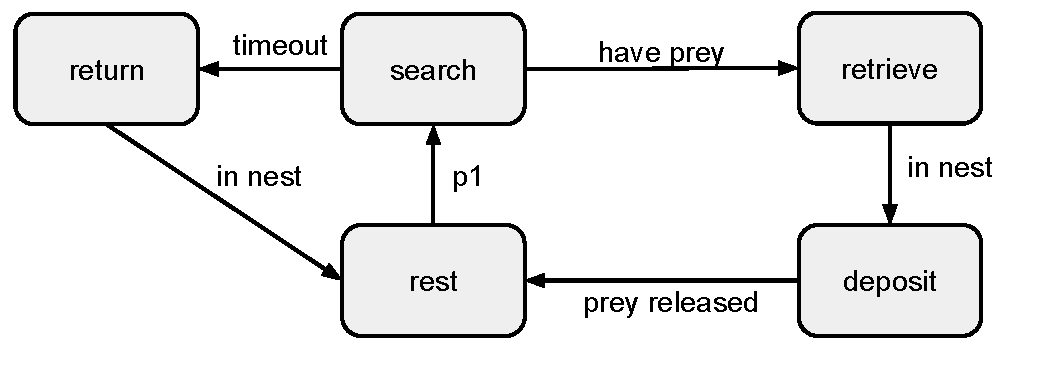
\includegraphics[width=\textwidth]{chapters/chapter2/figures/LabellaFSM.pdf}
\caption{Simplified finite state machine for Labella division of labour algorithm. }
\end{figure} 

Hoff \cite{hoff2010two} proposes a two ant-based foraging algorithm which do not require marking the physical environment. Instead, robots themselves become pheromone markers. The algorithms differ in the manner in which the beacon-to-pheromone role is chosen. 

Virtual pheromone algorithm functions as follows: Two pheromone trails are created - one trail from the source to the food and another trail from the source to the nest. The trail is created by robots: During execution, robots stop exploration and become pheromone beacons. The pheromone beacon robots simply broadcast a floating point number known as virtual pheromone. 
Local direct communications are used to transmit the virtual pheromone value.

The second technique uses cardinality where if a robot can hear 2 or more beacons then the robot stays a walker else the robot becomes a beacon. The advantage of using this technique over the other mentioned pheromone techniques is that robots are simpler due to simpler communication mechanisms as well as the lack of need for complex beacon deployment systems. Experiments are conducted with and without obstacles and a real-world simulator is used. The result show that congestion effects performance the most at high robot density. 

\subsubsection{Honey Bee Inspired Foraging Algorithms}
Bee swarms have been used in swarm robotics for problems such as path planning \cite{lin2009chaotic}, aggregation \cite{kernbach2009re}, collective perception \cite{schmickl2007collective}. Foraging algorithms have been developed that simulate a simplified honey bee recruitment in \cite{alers2014biologically}, which focuses on an actual robot demonstration of the technique using a turtle robot. Prior work focuses on implementing the same algorithm on e-pucks. 

The algorithm consists of two phases: an exploratory phase followed by an exploitive phase. Initially, all robots are located around the hive. In the exploratory phase, all robots perform a random search with a levy distribution until a food source is found by a robot. The exploitation phase begins where the robot that located the food returns to the hive and communicates the location to other members of the robot swarm. The other robots are recruited and begin to commute between the hive and the food source, transporting virtual food. This algorithm claims to exhibit three behaviours of bees: waiting around the hive, exploring the environment and foraging. Unlike bees, the algorithm used does not consider the division of labour between foragers, explorers and waiting robots, but rather uses an extremely simple model for bees which can only exploit a single food source. The robots use path integration in order to remember the location of the food source, and use a north-star type navigation in order to locate the hive. The path integration vector gets communicated to the other robots which use the vector to guide them to the food source. 

%%%%%%%%%%%%%%%%%%%%%%%%%%%%%%%%%%%%%%%%%%%%%%%%%

\subsection{Challenges in Swarm Robotic Foraging}
\label{challengesinforaging}
%TODO: Citations

Foraging for humans is a near trivial problem. Most children can walk around and retrieve blocks and return them to a single source. The seemingly simple sub-activities required by foraging such as identification and grasping are often relatively complex for robots to perform. Unlike other simpler, swarm robotics problems such as aggregation, foraging is made up of a group of non-trivial sub-tasks. Some of the aspects which are problematic for robots in a foraging are discussed below:

\begin{itemize}
\item Mechanically Challenging Interactions - Despite how far robotics has come as a field, there are still tasks that are trivial for humans, but still very complex for most robots. For instance, the challenge of picking up items \cite{saxena2008robotic} and moving them to another location requires high quality sensors, sensitive actuators and time-consuming calibration \cite{mondada2005cooperation}. 

\item Complex Noisy Environments - Although research can be performed in a controlled environment, for robust foraging to be efficiently applied in real-life, environmental factors have to be taken into consideration. Environmental factors such as light \cite{browning2005real,jungel2003real} and quality of the surface the robots forage on \cite{trianni2006cooperative}, often make a robotic solution complex, non-viable, non-robust or expensive. To cope with real-life environments, the robots require adaptive algorithms and more complex hardware for their sensors and actuators for basic navigation and object detection in unknown terrains with unknown lighting and weather conditions. 

\item Localization, Navigation and Obstacle Avoidance - Localization is the ability for a robot to depict their position in the environment. In swarm robotics, global knowledge about location (such as GPS) cannot be used by a robot to determine their position and where they are going. Non-trivial algorithms must be designed in order for a robot to position itself in the environment as ins \cite{zhou2012motion,rothermich2004distributed,arkin1992cooperation}. 

\end{itemize}

Swarm robotics researchers often choose to use simulated robot platforms such as Stage \cite{vaughan2008massively} or Argos \cite{pinciroli2011argos}, instead of real robots, in order to remove or regulate the amount of environmental noise. If a swarm robotics experiment uses real-life robots, the environments are usually simplified, by creating an environment where temperature, lighting and moisture are regulated\cite{labella2006division,nouyan2006group}. Due to the discussed complexities of foraging, existing swarm robotic research often simplifies the some of the complexities such as environmental changes, sensor noise, and the use of physical robots, in order to focus on a single aspect of foraging. 

%%%%%%%%%%%%%%%%%%%%%%%%%%%%%%%%%%%%%%%%%%%%%%%%%
%%%%%%%%%%%%%%%%%%%%%%%%%%%%%%%%%%%%%%%%%%%%%%%%%
\section{Summary}
\label{foraging:summary}

This chapter focused on reviewing foraging in nature and in swarm robotics as well as presenting a novel form of the foraging algorithm called prioritized foraging. 

In nature, social insects have efficient emergent foraging behaviours. Ants generally lay pheromone to guide the item search process, but the desert ant does not use pheromone and thus use a technique called path integration to relocate a food source. Honey bees employ more complex foraging behaviour including division of labour and communication. Winfield's foraging taxonomy is presented and discussed so that research can be contextualized in the field. 

Existing swarm robotics foraging algorithms are addressed and discussed under three sections: nature-inspired algorithm, standard foraging algorithms and multi foraging algorithms. Lastly, the novel idea of prioritized foraging is introduced. In prioritized foraging a particular item type has higher priority than other items. 

\chapter{Division of Labour}
\label{chap:divisionoflabour}


As explained in Section~\ref{flexibility}, division of labour forms part of foraging activities of social insects. This chapter defines division of labour as well as analyses different types of division of labour that occur in social insects. Lastly, division of labour strategies employed by different swarm robotics algorithms are described. 

\section{Definition of Division of Labour}
\label{sec:second:definition}

Oster et al. \cite{oster1978caste} defines division of labour as a ``stable pattern of variation" of the repertoire of tasks that individuals perform. Each individual specializes on a subset of the complete repertoire of tasks. The subset of the complete repertoire of tasks is called the specialization of an individual and the specialization of individuals varies across the swarm. 

Robinson et al. \cite{robinson1992regulation}, more simply, defines division of labour as the adjustment of ratios of workers engaged in different tasks based on external and internal stimuli.

There are two types of division of labour in social insects \cite{beshers2001models}: 
\begin{itemize}
	\item \textbf{Temporal polyethism} where the pattern of tasks being performed by a worker correlate to the age of the worker. In nature, the younger workers may perform tasks within the nest while the older workers perform tasks outside of the nest.
	\item \textbf{Morphological polyethism} where a worker with extreme physical features in terms of size or shape, will specialize more in particular tasks. The more extreme a particular physical feature is, the narrower the repertoire of the worker. For example, soldier ants are larger in order to defend the nest, while the smaller workers are involved with foraging.
\end{itemize}

%NEED SOMETHING HERE

%include if we find we need. for now, you're done
%\subsubsection{Task Selection}
%Before addressing the different models of division of labour, it's important to discuss one of the main distringuishing characteristics of division of labour: How does an individual select tasks? Much of the study of division of labour is related to how workers select tasks. The factors contributing to the decision are divided into internal and external factors. Internal factors refer to neurological, hormonal, experience or genetic factors where as the external factors refer to environmental stimuli, worker to worker interaction and communication of the increasing need of workers assigned to a particular task. \cite{beshers2001models}.

%Research around task selection is focused around the following topics: 
%\begin{itemize}
%	\item The rules guiding the decision process in workers
%	\item The process of how information about the environment and social stimuli is gathered
%	\item The internal choice mechanism for making the decisions
%\end{itemize}

\section{Models of Division of Labour from Biology}

An overview of existing models from entomology is provided in this section, since insect-like division of labour is used by the algorithms developed in this thesis. The section focuses on common models and models used by the algorithms described in this thesis.

\subsection{Response Threshold Model}
\label{responsethresholdmodel}

The response threshold model is where individuals each have a response threshold for each specific tasks that individuals in the swarm can perform.  The task-specific thresholds vary across individuals in the swarm \cite{robinson1989genetic}.

Suppose $R$ is the set of tasks that can be performed by individuals of the swarm. An individual $\gamma$ will only perform task $\nu \in R$ when the environmental stimuli for task $\nu$, $S_\nu$, exceeds the response threshold, $r_{\gamma,\nu}$, for task $\nu$, for an individual $\gamma$. Each response threshold for a task, for an individual is constant. If an individual has a lower threshold for a specific task, compared to other individuals in the swarm, then it is likely that the individual will become a specialist in that task \cite{robinson1989genetic}

Response threshold models have been modelled formally by Page et al. \cite{page1990self} and Bonabeau et al. \cite{bonabeau1999role}. Response thresholds have been used to explain temporal polyethism in honey bees where the response thresholds of the honey bees would change as the honey bees age \cite{robinson1987regulation}.

\subsection{Foraging for Work}

Foraging for work assumes that individuals are intrinsically identical and thus performance of individuals at a task is dependent on opportunity to perform a task, rather than intrinsic task preferences \cite{franks1994foraging}.

Foraging for work has two main principles:
\begin{enumerate}
	\item Individuals repeat the same task when possible.
	\item Individuals actively seek work when they have no task.
\end{enumerate}

%This forms the basic model of foraging and also is used in MY honey bee algorithm.

Foraging for work also assumes that tasks are radially spatially localized within the nest. This means that  tasks further away from the nest are performed by older individuals and the younger individuals perform the tasks that are closer the nest \cite{tofts1993algorithms}.

Foraging for work shows that temporal polyethism does not require age-related differences in the mechanism of task choice and can simply stem from an individual's proximity to the nest. Foraging for work is controversial since it shows that task organization might occur within a social group in absence of selection efforts or intrinsic mechanism of task performance \cite{franks1994foraging}. 

Foraging for work can be seen as a special case of the threshold model where all individuals have identical thresholds. In foraging for work, temporal polyethism is generated by spatial organisation, where as response threshold model generate temporal polyethism by differences in internal thresholds. Unlike response threshold models, foraging for work does not suffer from inactive individuals as all workers are either performing or seeking tasks \cite{beshers2001models}.

Foraging for work is controversial in the fact that it induces division of labour without any explicit mechanism, but instead as a natural result of the environment \cite{beshers2001models}. However, it has been shown that in insect colonies, there is intrinsic variation in each individuals' response to environmental  stimuli, rather than from opportunity alone \cite{julian1999undertaking}.

\subsection{Self Reinforcement Models}
\label{selfreinforcement}

% What are self reinforceme models citation
Self reinforcement models adjust an individual's probability of performing a task, based on prior success or failure to perform that task. Initially, the probability of performing all tasks are equal. If a task is performed successfully or there is  no opportunity to perform a task, then the probability of performing that task again is reduced. Individuals that continuously successfully perform a specific task become specialists in that task. Task success is directly proportional of the probability of doing the task again \cite{theraulaz1998response, pasteels1987individual}. Self reinforcement has been attributed for division of labour in many systems in nature \cite{spencer1998dynamics}%citations

% More details?
    
%NB: ABOVE is what happens in my own things
% IS IT?! Will have to check

\subsection{Social Inhibition Models}
With social inhibition models, individuals change tasks as they age, however the process of aging is inhibited by social environments \cite{huang1992honeybee}. The model is based on the activator-inhibitor behaviour present in bee swarms. 

In honey bee swarm, juvenile bees work in the hive while an older bee forages. When a juvenile bee develops, it becomes a forager bee. The activator hormone motivates growth of a juvenile bee into a forager bee \cite{robinson1989genetic}. An inhibitor hormone is released by the forager bees which is transferred to the juvenile worker bees. The inhibitor hormone inhibits the development of a juvenile bee into a forager bee \cite{huang1992honeybee}.

The existence of forager bees in the hive slows the development process of the juvenile bees and thus the juvenile bees remain workers. If forager bees are destroyed, then less inhibitor hormone is released and more worker bees become forager bees, replenishing the number of foragers. 

                                
\subsection{Network Models of Task Allocation}

Network models assume that swarm individuals are identical and that division of labour is induced by effective communication of the number of individuals required per task, between individuals of the swarm \cite{gordon1992parallel}. A number of network models exist \cite{gordon1992parallel,pacala1996effects}.

Network models are similar to foraging for work models in that division of labour is generated by changes in local information encountered by each individual, rather than by intrinsic differences in individuals. 


\section{Division of Labour in Robot Swarms}

Division of labour has been used in swarm robotics. This section provides an overview of the use of division of labour in swarm robotics.

Agassounon et al. \cite{agassounon2002efficiency} design and demonstrate three response threshold-based methods for division of labour. Response threshold model is described in Section~\ref{responsethresholdmodel}. The robots had to perform a clustering task with multiple sites. The task choice was to select which site to cluster. Division of labour techniques were employed to avoid interference between robots that occurs more often when too many robots attempt to cluster the same site. 

The experiment determined that the swarm benefited from threshold division of labour since the algorithms with division of labour performed similarly or better than those with a fixed task group size. The experiment also determined that local communication improved swarm performance.

Labella et al. \cite{labella2006division} developed a division of labour strategy for prey retrieval based on Deneubourg's ant self re-enforcement model, discussed in Section~\ref{selfreinforcement}. Experimentation was performed on simulated and real robots. The Robots switched from search behaviour to rest behaviour with probability $z$. This probability was incremented by a delta when a robot successfully returned to the nest with an item and decremented by the same delta when a robot returns to the nest without an item. Labella et al. classified the foragers into different types, loafers, foragers or  undecided, based on the final value of $z$. Experiments showed that the values of $z$ tended towards extreme values, showing that, robots tended to become either loafers or foragers, while only a few became undecided. It was shown that a simple self-reinforcement division of labour model can improve the performance of a swarm of robots at a task, without the need for communication. However scalability was still a concern, since the swarm experienced negative performance as swarm size increased. 

Liu et al. \cite{liu2007towards} introduce three mechanisms for adapting the number of resting robots to foraging robots in a simple foraging problem. The mechanisms consist of variations on how one perceives the worker demand. The mechanisms were as follows:

\begin{itemize}
	\item The internal success of an individual at a specific task.
	\item The collective success of the swarm at a specific task. 
	\item  The amount of environmental interference experienced by an individual while performing a task, most importantly the amount of collisions with other robots. This technique is a social inhibition model.
\end{itemize}

The mechanisms are used to adjust time specific thresholds related to the length of time to wait before returning to work and how long work should be performed for.
Four combinations of these factors are evaluated as well as compared to a nai\"ve foraging approach. The performance of the swarm is measured as the energy spent by a robot. The efficiency is evaluated over different robot quantities and food densities.

The experiments discovered that the use of the mechanisms improved performance significantly compared to swarms without such mechanisms. It was also shown that the mechanisms resulted in emergent division of labour, regulating the number of foraging and resting robots. The experiments resulted in robustness in environmental changes related to the density of items. The experiments using collective success of the swarm achieved the highest net energy income to the swarm and also had the fastest adaptation of the ratio of foragers to resting robots, when food density changes. Liu et al. \cite{liu2007towards} notes that scalability was not tested in the experiments.

By examining the existing swarm robot division of labour literature, one can conclude that the majority of research in division of labour for swarm robotics, is concerned with regulating the number of active robots in a swarm. The existing research shows that the ability of a swarm to adjust the amount of robots actively participating in a task with the amount of robots at rest, enables the swarm to adapt to changes in the environment. Existing research also concluded that division of labour improved swarm robustness to destruction of robots, by replenishing the number of active robots when active robots had been removed. There exists scope to investigate division of labour between multiple different active tasks. This thesis addresses division of labour between two active tasks, contrasting the most division of labour research.

The existing research did not test scalability of the division of labour techniques, since the maximum swarm size was usually 10 or less. This thesis will evaluate the scalability of division of labour techniques used. There exists scope for investigating other types of division of labour in swarm robotics, such as network models, but is not the scope of this thesis.


\section{Summary}
\label{sec:second:summary}
Division of labour is the adjustment of ratios of workers engaged in different tasks, based on external and internal stimuli. Division of labour is used in social insect societies such as bees and ants. Multiple models for division of labour have been explored by biologists. Extensive research has been performed about response threshold models, foraging for work, network models and self-reinforcement models. Despite the large amount of models, little verification of these models have been performed in real or simulated environments. 

The use of division of labour in swarm robotics was reviewed. Most of the reviewed research was focused around the problem of using division of labour to regulate the number of active robots to the number of inactive robots. The techniques used in swarm robotics employ a variety of division of labour models such as response threshold models, self re-enforcement and social inhibition models. 

The author notes that the reviewed research did not adequately address the scalability of the techniques.
